% Uebung Nr. 7 Zeigerdiagramm nach Brinkmeyer
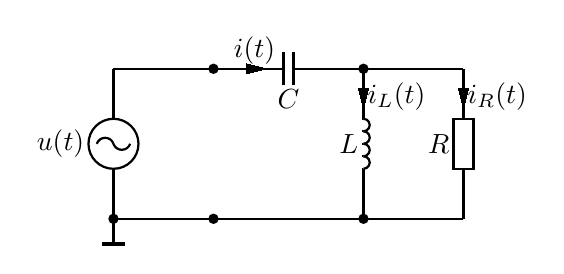
\begin{tikzpicture}[scale=2.54]%
% dpic version 2024.01.01 option -g for TikZ and PGF 1.01
\ifx\dpiclw\undefined\newdimen\dpiclw\fi
\global\def\dpicdraw{\draw[line width=\dpiclw]}
\global\def\dpicstop{;}
\dpiclw=0.8bp
\dpiclw=0.8bp
\dpicdraw (0,0)
 --(0,-0.25)\dpicstop
\dpicdraw (0,-0.375) circle (0.049213in)\dpicstop
\dpicdraw (-0,-0.375)
 ..controls (-0.005978,-0.357065) and (-0.022762,-0.344968)
 ..(-0.041667,-0.344968)
 ..controls (-0.060571,-0.344968) and (-0.077355,-0.357065)
 ..(-0.083333,-0.375)\dpicstop
\dpicdraw (0,-0.375)
 ..controls (0.005978,-0.392935) and (0.022762,-0.405032)
 ..(0.041667,-0.405032)
 ..controls (0.060571,-0.405032) and (0.077355,-0.392935)
 ..(0.083333,-0.375)\dpicstop
\dpicdraw (0,-0.5)
 --(0,-0.75)\dpicstop
\draw (-0.125,-0.375) node[left=-2bp]{$ u(t)$};
\dpicdraw[fill=black](0,-0.75) circle (0.007874in)\dpicstop
\dpicdraw (0,-0.75)
 --(0,-0.875)\dpicstop
\dpicdraw[line width=1.6bp](0.055556,-0.875)
 --(-0.055556,-0.875)\dpicstop
\dpicdraw (0,0)
 --(0.5,0)\dpicstop
\dpicdraw[fill=black](0.5,0) circle (0.007874in)\dpicstop
\dpicdraw[fill=black](0.5,-0.75) circle (0.007874in)\dpicstop
\dpicdraw (0.5,0)
 --(0.85,0)\dpicstop
\dpicdraw (0.85,-0.083333)
 --(0.85,0.083333)\dpicstop
\dpicdraw (0.9,-0.083333)
 --(0.9,0.083333)\dpicstop
\dpicdraw (0.9,0)
 --(1.25,0)\dpicstop
\draw (0.875,-0.083333) node[below=-2bp]{$ C$};
\filldraw[line width=0bp](0.666667,-0.025)
 --(0.766667,0)
 --(0.666667,0.025) --cycle\dpicstop
\dpicdraw (0.743761,0)
 --(0.666667,0)\dpicstop
\draw (0.705214,0) node[above=-2bp]{$ i(t) $};
\dpicdraw[fill=black](1.25,0) circle (0.007874in)\dpicstop
\dpicdraw (1.25,0)
 --(1.25,-0.25)\dpicstop
\dpicdraw (1.25,-0.25)
 --(1.244444,-0.25)\dpicstop
\dpicdraw (1.25,-0.25)
 ..controls (1.261165,-0.25) and (1.271481,-0.255956)
 ..(1.277063,-0.265625)
 ..controls (1.282646,-0.275294) and (1.282646,-0.287206)
 ..(1.277063,-0.296875)
 ..controls (1.271481,-0.306544) and (1.261165,-0.3125)
 ..(1.25,-0.3125)\dpicstop
\dpicdraw (1.25,-0.3125)
 --(1.244444,-0.3125)\dpicstop
\dpicdraw (1.25,-0.3125)
 ..controls (1.261165,-0.3125) and (1.271481,-0.318456)
 ..(1.277063,-0.328125)
 ..controls (1.282646,-0.337794) and (1.282646,-0.349706)
 ..(1.277063,-0.359375)
 ..controls (1.271481,-0.369044) and (1.261165,-0.375)
 ..(1.25,-0.375)\dpicstop
\dpicdraw (1.25,-0.375)
 --(1.244444,-0.375)\dpicstop
\dpicdraw (1.25,-0.375)
 ..controls (1.261165,-0.375) and (1.271481,-0.380956)
 ..(1.277063,-0.390625)
 ..controls (1.282646,-0.400294) and (1.282646,-0.412206)
 ..(1.277063,-0.421875)
 ..controls (1.271481,-0.431544) and (1.261165,-0.4375)
 ..(1.25,-0.4375)\dpicstop
\dpicdraw (1.25,-0.4375)
 --(1.244444,-0.4375)\dpicstop
\dpicdraw (1.25,-0.4375)
 ..controls (1.261165,-0.4375) and (1.271481,-0.443456)
 ..(1.277063,-0.453125)
 ..controls (1.282646,-0.462794) and (1.282646,-0.474706)
 ..(1.277063,-0.484375)
 ..controls (1.271481,-0.494044) and (1.261165,-0.5)
 ..(1.25,-0.5)\dpicstop
\dpicdraw (1.25,-0.5)
 --(1.244444,-0.5)\dpicstop
\dpicdraw (1.25,-0.5)
 --(1.25,-0.75)\dpicstop
\draw (1.244444,-0.375) node[left=-2bp]{$ L$};
\filldraw[line width=0bp](1.225,-0.1)
 --(1.25,-0.2)
 --(1.275,-0.1) --cycle\dpicstop
\dpicdraw (1.25,-0.177094)
 --(1.25,-0.1)\dpicstop
\draw (1.25,-0.138547) node[right=-2bp]{$ i_L(t) $};
\dpicdraw[fill=black](1.25,-0.75) circle (0.007874in)\dpicstop
\dpicdraw (1.25,0)
 --(1.75,0)\dpicstop
\dpicdraw (1.75,0)
 --(1.75,-0.25)\dpicstop
\dpicdraw (1.75,-0.5)
 --(1.8,-0.5)
 --(1.8,-0.25)
 --(1.7,-0.25)
 --(1.7,-0.5)
 --(1.75,-0.5)\dpicstop
\dpicdraw (1.75,-0.5)
 --(1.75,-0.75)\dpicstop
\draw (1.7,-0.375) node[left=-2bp]{$ R$};
\filldraw[line width=0bp](1.725,-0.1)
 --(1.75,-0.2)
 --(1.775,-0.1) --cycle\dpicstop
\dpicdraw (1.75,-0.177094)
 --(1.75,-0.1)\dpicstop
\draw (1.75,-0.138547) node[right=-2bp]{$ i_R(t) $};
\dpicdraw (1.75,-0.75)
 --(0,-0.75)\dpicstop
\end{tikzpicture}%
